\documentclass{../kin_math}

\header{Elijah Kin}{Homework 13}{AMSC660}
\headrule

\begin{document}

\begin{questions}
  \question Consider the classification problem \texttt{one} versus \texttt{seven} with the MNIST dataset from the previous homework. Use the same settings as for the stochastic gradient descent, i.e., the quadratic dividing hypersurface
  \begin{equation*}
    x^\top W x + v^\top x + b,
  \end{equation*}
  the quadratic test function
  \begin{equation*}
    q(x_j; \textbf{w}) \coloneqq y_j\left(x^\top W x + v^\top x + b\right),
  \end{equation*}
  and the loss function
  \begin{equation*}
    f(\textbf{w}) = \frac{1}{n} \sum_{j = 1}^n \log\left(1 + e^{-q(x_j; \textbf{w})}\right) + \frac{\lambda}{2} \lVert \textbf{w} \rVert^2.
  \end{equation*}
  Here \textbf{w} denotes the $d^2 + d + 1$-dimensional vector of coefficients of $\{W, v, b\}$.

  Implement
  \begin{enumerate}
    \item Deterministic and Stochastic Nesterov (experiment with various batch sizes). Its deterministic version is given by Eqs. (61)-(62) in \texttt{Optimization.pdf};
    \item Deterministic and Stochastic Adam (experiment with various batch sizes). Its deterministic version is proposed in a paper by D. P. Kingma and J. L. Ba ``Adam: A Method for Stochastic Optimization'' where ADAM is introduced: \url{https://arxiv.org/pdf/1412.6980.pdf}.
  \end{enumerate}
  You can use a constant step size. Run the stochastic optimizers for the same number of epochs (if you have $n$ data points and your batch size is $m$ then $\textsf{round}(n / m)$ timesteps is one epoch). Compare the performance of these optimizers with each other and with the stochastic gradient descent from the previous homework. Write a report containing graphs of the objective function and the norm of its gradient versus the iteration number. Which stochastic optimizer do you find the most efficient? Which batch size do you recommend? Which step size do you recommend?
  \begin{solution}
    TODO
  \end{solution}

  \question Consider the KKT system
  \begin{equation*}
    \begin{bmatrix} G & A^\top \\ A & 0 \end{bmatrix} \begin{bmatrix} -\textbf{p} \\ \boldsymbol{\lambda} \end{bmatrix} = \begin{bmatrix} \textbf{g} \\ 0 \end{bmatrix}
  \end{equation*}
  where $G$ is $d \times d$ symmetric positive definite and $A$ is $m \times d$ and has linearly independent rows. Show that the matrix
  \begin{equation*}
    K \coloneqq \begin{bmatrix} G & A^\top \\ A & 0 \end{bmatrix}
  \end{equation*}
  is of \emph{saddle-point type}, i.e., it has $d$ positive eigenvalues and $m$ negative ones. \emph{Hint: Find matrices $X$ and $S$ ($S$ is called the \textbf{Schur complement}) such that
  \begin{equation*}
    \begin{bmatrix} G & A^\top \\ A & 0 \end{bmatrix} = \begin{bmatrix} I & 0 \\ X & I \end{bmatrix} \begin{bmatrix} G & 0 \\ 0 & S \end{bmatrix} \begin{bmatrix} I & X^\top \\ 0 & I \end{bmatrix}.
  \end{equation*}
  Then use Sylvester's law of inertia (look it up!) to finish the proof.}
  \begin{solution}
    Starting with the ansatz suggested by the hint, note that
    \begin{equation*}
      \begin{bmatrix} I & 0 \\ X & I \end{bmatrix} \begin{bmatrix} G & 0 \\ 0 & S \end{bmatrix} \begin{bmatrix} I & X^\top \\ 0 & I \end{bmatrix} = \begin{bmatrix} G & 0 \\ XG & S \end{bmatrix} \begin{bmatrix} I & X^\top \\ 0 & I \end{bmatrix} = \begin{bmatrix} G & GX^\top \\ XG & XGX^\top + S \end{bmatrix}
    \end{equation*}
    hence to achieve equality with $K$ in the bottom left block, let $X = AG^{-1}$. It remains to achieve equality in the bottom right block; note that
    \begin{equation*}
      XGX^\top + S = AG^{-1} G (AG^{-1})^\top + S = AG^{-1}A^\top + S
    \end{equation*}
    and hence we take $S = -AG^{-1}A^\top$ to achieve equality with $K$. Hence, we have written
    \begin{equation*}
      K = \begin{bmatrix} I & 0 \\ X & I \end{bmatrix} \begin{bmatrix} G & 0 \\ 0 & S \end{bmatrix} \begin{bmatrix} I & 0 \\ X & I \end{bmatrix}^\top.
    \end{equation*}
    Since $K$ is symmetric (because $G$ is symmetric), by Sylvester's law of inertia, we have that $K$ has the same inertia as the symmetric matrix
    \begin{equation*}
      \begin{bmatrix}
        G & 0 \\ 0 & S
      \end{bmatrix}.
    \end{equation*}
    We now claim that the eigenvalues of the above matrix are exactly the eigenvalues of $G$ and $S$ combined. This follows from the multiplicativity of the determinant, since,
    \begin{multline*}
      \det\left(\begin{bmatrix} G - \lambda I_d & 0 \\ 0 & S - \lambda I_m \end{bmatrix}\right) = \det\left(\begin{bmatrix} G - \lambda I_d & 0 \\ 0 & I_m \end{bmatrix} \begin{bmatrix} I_d & 0 \\ 0 & S - \lambda I_m \end{bmatrix}\right) \\
      = \det\left(\begin{bmatrix} G - \lambda I_d & 0 \\ 0 & I_m \end{bmatrix}\right) \det\left(\begin{bmatrix} I_d & 0 \\ 0 & S - \lambda I_m \end{bmatrix}\right) = \det\left(G - \lambda I_d\right) \det\left(S - \lambda I_m\right).
    \end{multline*}
    Hence, the characteristic polynomial of the above matrix is the product of the characteristic polynomials of $G$ and $S$, so the eigenvalues of the above matrix are exactly the eigenvalues of $G$ and $S$ combined.

    It remains to show that all $m$ eigenvalues of $S$ are negative. Toward this end, consider
    \begin{equation*}
      x^\top S x = -x^\top AG^{-1} A^\top x = -(A^\top x)^\top G^{-1} (A^\top x).
    \end{equation*}
    Then since $G^{-1}$ is symmetric positive definite,
    \begin{equation*}
      x^\top S x = -(A^\top x)^\top G^{-1} (A^\top x) \leq 0
    \end{equation*}
    with equality if and only if $A^\top x = 0$, hence $S$ is negative definite, meaning all eigenvalues of $S$ are negative. Hence, referring back to Sylvester's law of inertia, $K$ has $d$ positive eigenvalues and $m$ negative ones.
  \end{solution}

  \question Consider an equality-constrained quadratic program QP
  \begin{align*}
    &\min \frac{1}{2} \textbf{x}^\top G \textbf{x} + \textbf{c}^\top \textbf{x} \\
    &\text{subject to } A \textbf{x} = \textbf{b}.
  \end{align*}
  The matrix $G$ is symmetric. Assume that $A$ is full rank (i.e., its rows are linearly independent) and $Z^\top GZ$ is positive definite where $Z$ is a basis for the null-space of $A$, i.e., $AZ = 0$.
  \begin{enumerate}
    \item Write the KKT system for this case in the matrix form.
    \begin{solution}
      From the above, we define the Lagrangian
      \begin{equation*}
        \mathcal{L}(\textbf{x}, \boldsymbol{\lambda}) = \frac{1}{2} \textbf{x}^\top G \textbf{x} + \textbf{c}^\top \textbf{x} - \boldsymbol{\lambda}^\top (A\textbf{x} - \textbf{b})
      \end{equation*}
      in which case
      \begin{equation*}
        \nabla_\textbf{x} \mathcal{L} = G \textbf{x} + \textbf{c} - A^\top \boldsymbol{\lambda}.
      \end{equation*}
      Taking $\nabla_\textbf{x} \mathcal{L} = 0$, we obtain the system
      \begin{align*}
        G \textbf{x} + \textbf{c} - A^\top \boldsymbol{\lambda} &= 0 \\
        A \textbf{x} - \textbf{b} &= 0
      \end{align*}
      which we can rewrite as
      \begin{align*}
        G (-\textbf{x}) + A^\top \boldsymbol{\lambda} &= \textbf{c} \\
        A (-\textbf{x}) &= - \textbf{b}
      \end{align*}
      or equivalently,
      \begin{align*}
        \begin{bmatrix} G & A^\top \\ A & 0 \end{bmatrix} \begin{bmatrix} -\textbf{x} \\ \boldsymbol{\lambda} \end{bmatrix} = \begin{bmatrix} \textbf{c} \\ -\textbf{b} \end{bmatrix}.
      \end{align*}
    \end{solution}
    \item Show that the matrix of this system $K$ is invertible. \emph{Hint: assume that there is a vector $\textbf{z} \coloneqq (\textbf{x}, \textbf{y})^\top$ such that $K \textbf{z} = 0$. Consider the quadratic form $\textbf{z}^\top K \textbf{z}$, use logical reasoning and algebra, and arrive at the conclusion that then $\textbf{z} = 0$.}
    \begin{solution}
      From (a), recall that
      \begin{equation*}
        K = \begin{bmatrix} G & A^\top \\ A & 0 \end{bmatrix}
      \end{equation*}
      and so for arbitrary $\textbf{z} \coloneqq (\textbf{x}, \textbf{y})^\top$ it follows that
      \begin{multline*}
        \textbf{z}^\top K \textbf{z} = \begin{bmatrix} \textbf{x}^\top & \textbf{y}^\top \end{bmatrix} \begin{bmatrix} G & A^\top \\ A & 0 \end{bmatrix} \begin{bmatrix} \textbf{x} \\ \textbf{y} \end{bmatrix} = \textbf{x}^\top (G \textbf{x} + A^\top \textbf{y}) + \textbf{y}^\top A \textbf{x} \\
        = \textbf{x}^\top G \textbf{x} + \textbf{x}^\top A^\top \textbf{y} + \textbf{y}^\top A \textbf{x}.
      \end{multline*}
      Further, since $\textbf{x}^\top A^\top \textbf{y}$ is a scalar,
      \begin{equation*}
        \textbf{x}^\top A^\top \textbf{y} = (\textbf{x}^\top A^\top \textbf{y})^\top = \textbf{y}^\top A \textbf{x}
      \end{equation*}
      and so
      \begin{equation}
        \label{eq:arbitrary}
        \textbf{z}^\top K \textbf{z} = \textbf{x}^\top G \textbf{x} + 2 \textbf{y}^\top A \textbf{x}.
      \end{equation}
      Now assume that $\textbf{z}$ is such that $K \textbf{z} = 0$. Then
      \begin{equation*}
        0 = K \textbf{z} = \begin{bmatrix} G & A^\top \\ A & 0 \end{bmatrix} \begin{bmatrix} \textbf{x} \\ \textbf{y} \end{bmatrix} = \begin{bmatrix} G \textbf{x} + A^\top \textbf{y} \\ A \textbf{x} \end{bmatrix},
      \end{equation*}
      so we have both that $G \textbf{x} + A^\top \textbf{y} = 0$ and $A \textbf{x} = 0$. Further, $\textbf{z}^\top K \textbf{z} = \textbf{z}^\top (0) = 0$. Substituting these facts into (\ref{eq:arbitrary}), we find that
      \begin{equation*}
        0 = \textbf{z}^\top K \textbf{z} = \textbf{x}^\top G \textbf{x} + 2 \textbf{y}^\top A \textbf{x} = \textbf{x}^\top G \textbf{x} + 2 \textbf{y}^\top(0) = \textbf{x}^\top G \textbf{x}
      \end{equation*}
      and so $\textbf{x}^\top G \textbf{x} = 0$.

      Now let $Z$ be a basis for the null-space of $A$. In particular, since $A \textbf{x} = 0$, we can write $\textbf{x} = Z \hat{\textbf{x}}$, a linear combination of the columns of $Z$. Then
      \begin{equation*}
        0 = \textbf{x}^\top G \textbf{x} = (Z \hat{\textbf{x}})^\top G (Z \hat{\textbf{x}}) = \hat{\textbf{x}}^\top (Z^\top G Z) \hat{\textbf{x}}.
      \end{equation*}
      Hence, since $\hat{\textbf{x}}^\top (Z^\top G Z) \hat{\textbf{x}} = 0$ and $Z^\top G Z$ is assumed to be positive definite, it must be that $\hat{\textbf{x}} = 0$, and likewise, $\textbf{x} = Z \hat{\textbf{x}} = 0$.

      It remains to show that $\textbf{y} = 0$ also. This follows from
      \begin{equation*}
        0 = G \textbf{x} + A^\top \textbf{y} = A^\top \textbf{y}
      \end{equation*}
      and the fact that $A$ has linearly independent rows, so $A^\top$ has linearly independent columns, meaning $\textbf{y} = 0$ since $A^\top \textbf{y} = 0$.

      Hence, $K \textbf{z} = 0$ has only the trivial solution $\textbf{z} = 0$, meaning $K$ is invertible.
    \end{solution}
    \item Conclude that there exists a unique vector $(\textbf{x}^*, \boldsymbol{\lambda}^*)^\top$ that solves the KKT system. Note that since we have only equality constraints, the positivity of $\boldsymbol{\lambda}$ is irrelevant.
    \begin{solution}
      Since $K$ is invertible, we can simply recover the vector by taking
      \begin{equation*}
        K^{-1} \begin{bmatrix} \textbf{c} \\ -\textbf{b} \end{bmatrix}.
      \end{equation*}
    \end{solution}
  \end{enumerate}

  \question Consider the following quadratic program with inequality constraints:
  \begin{align*}
    &\min f(x, y) = (x - 1)^2 + (y - 2.5)^2 \\
    &\text{subject to } x - 2y + 2, -x - 2y + 6, -x + 2y + 2, x, y \geq 0
  \end{align*}
  \begin{enumerate}
    \item Plot the level sets of the objective function and the feasible set.
    \begin{solution}
      We plot the level sets of the objective function and the boundary of the feasible set below. The corresponding code can be found \href{https://github.com/elijahkin/amsc660/blob/main/hw13/hw13.ipynb}{here}.
      \begin{figure}
        \centering
        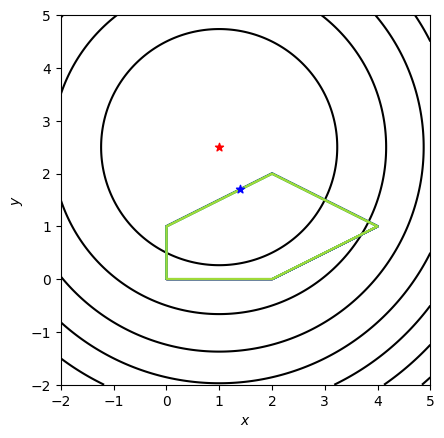
\includegraphics[scale=0.8]{feasible.png}
      \end{figure}
    \end{solution}
    \item What is the exact solution? Find it analytically with the help of your figure.
    \begin{solution}
      From the above figure, we see that solution lies on the line $x - 2y + 2 = 0$. Solving for $x$, we find $x = 2y - 2$, and so we seek to find
      \begin{equation*}
        \min f(2y - 2, y) = \min (2y - 3)^2 + (y - 2.5)^2
      \end{equation*}
      which occurs where
      \begin{equation*}
        0 = \frac{d}{dy} \left[(2y - 3)^2 + (y - 2.5)^2\right] = 4(2y - 3) + 2(y - 2.5) = 10y - 17,
      \end{equation*}
      so $y^* = 17 / 10$ and hence $x^* = 14 / 10$.
    \end{solution}
    \item Suppose the initial point is $(2, 0)$. Initially, constraints 3 and 5 are active, hence start with $\mathcal{W} = \{3, 5\}$. Work out all iterations of the active-set method analytically. The arising linear systems should be very easy to solve. For each iteration, you need to write out the set $\mathcal{W}$, the KKT system, its solution, i.e., $(p_x, p_y)$, the vector of Lagrange multipliers, and the current iterate $(x_k, y_k)$. Plot all iterates on your figure. There should be a total of 5 iterations.
    \begin{solution}
      TODO
    \end{solution}
  \end{enumerate}
\end{questions}

\end{document}
